\section{Analysis and Interpretation}
The main interpretation is that participant groups differ in how residual gaze costs
respond to contextual predictability. Because residual gaze features are computed from
held-out participant rows after residual models are fit only on training participants,
the profile is not a direct copy of the label or a random word-level split artifact.
The exposure-only comparison rejects the simpler explanation that participants are
separated merely by reading different text. The primary model also excludes direct
exposure-count variables, and raw-speed/global-duration features are not the selected
feature family.

Feature stability supports this interpretation: the stable features are DFM residual
gaze slopes rather than direct row-count or speech-count variables
(Table~\ref{tab:feature-stability}, Figure~\ref{fig:feature-stability}). Focused
reader-group interactions provide interpretability rather than the central claim. DFM
surprisal interactions provide the strongest explanatory support, word-length
interactions provide secondary support, and previous-boundary opacity is retained as a
secondary interpretability feature (Table~\ref{tab:interaction-synthesis},
Figure~\ref{fig:interaction-summary}). Text-exposure audits are shown in
Figure~\ref{fig:text-exposure-audit}. The claim ledger in
Table~\ref{tab:claims-evidence} defines which results are main, secondary,
appendix-only, deferred, or dropped.

\begin{table}[t]
\centering
\small
\caption{Stable standardized coefficients for the locked final model.}
\label{tab:feature-stability}
\begin{tabular}{llllll}
\toprule
feature\_group & feature & mean\_coefficient & sd\_coefficient & n\_folds & positive\_rate \\
\midrule
D3\_dfm\_residual\_gaze\_only & crossfit\_total\_fixation\_residual\_dfm\_entropy\_slope & 1.0863 & 0.0641 & 57 & 1.0000 \\
D3\_dfm\_residual\_gaze\_only & crossfit\_first\_pass\_residual\_dfm\_entropy\_slope & 0.9849 & 0.0430 & 57 & 1.0000 \\
D3\_dfm\_residual\_gaze\_only & crossfit\_go\_past\_residual\_dfm\_surprisal\_slope & 0.9177 & 0.0496 & 57 & 1.0000 \\
D3\_dfm\_residual\_gaze\_only & crossfit\_fixation\_count\_residual\_dfm\_surprisal\_slope & 0.6404 & 0.0599 & 57 & 1.0000 \\
D3\_dfm\_residual\_gaze\_only & crossfit\_total\_fixation\_residual\_dfm\_surprisal\_slope & 0.5938 & 0.0606 & 57 & 1.0000 \\
D3\_dfm\_residual\_gaze\_only & crossfit\_ffd\_residual\_dfm\_entropy\_slope & -0.5886 & 0.0682 & 57 & 0.0000 \\
D3\_dfm\_residual\_gaze\_only & crossfit\_go\_past\_residual\_dfm\_entropy\_slope & 0.1970 & 0.0535 & 57 & 1.0000 \\
D3\_dfm\_residual\_gaze\_only & crossfit\_fixation\_count\_residual\_dfm\_entropy\_slope & -0.1904 & 0.0532 & 57 & 0.0175 \\
D3\_dfm\_residual\_gaze\_only & crossfit\_skipping\_residual\_dfm\_entropy\_slope & 0.1596 & 0.0489 & 57 & 1.0000 \\
D3\_dfm\_residual\_gaze\_only & crossfit\_skipping\_residual\_dfm\_surprisal\_slope & 0.1298 & 0.0481 & 57 & 0.9825 \\
D3\_dfm\_residual\_gaze\_only & crossfit\_ffd\_residual\_dfm\_surprisal\_slope & -0.1229 & 0.0684 & 57 & 0.0526 \\
D3\_dfm\_residual\_gaze\_only & crossfit\_first\_pass\_residual\_dfm\_surprisal\_slope & 0.0911 & 0.0460 & 57 & 0.9474 \\
\bottomrule
\end{tabular}
\end{table}

\begin{table}[t]
\centering
\small
\caption{Focused reader-group interaction synthesis.}
\label{tab:interaction-synthesis}
\begin{tabular}{llllll}
\toprule
phase4\_interaction & outcome & estimate & std\_error & p\_value & survives\_controls \\
\midrule
reader\_group\_x\_word\_length & log\_ffd & -0.0152 & 0.0045 & 0.0007 & True \\
reader\_group\_x\_dfm\_surprisal & log\_ffd & 0.0043 & 0.0045 & 0.3405 & False \\
reader\_group\_x\_previous\_boundary\_opacity & log\_ffd & -0.0031 & 0.0022 & 0.1530 & False \\
reader\_group\_x\_word\_length & log\_first\_pass\_duration & 0.0075 & 0.0148 & 0.6127 & False \\
reader\_group\_x\_dfm\_surprisal & log\_first\_pass\_duration & 0.0179 & 0.0070 & 0.0110 & True \\
reader\_group\_x\_previous\_boundary\_opacity & log\_first\_pass\_duration & -0.0048 & 0.0029 & 0.0945 & False \\
reader\_group\_x\_word\_length & log\_go\_past\_time & 0.0230 & 0.0187 & 0.2183 & False \\
reader\_group\_x\_dfm\_surprisal & log\_go\_past\_time & 0.0292 & 0.0098 & 0.0029 & True \\
reader\_group\_x\_previous\_boundary\_opacity & log\_go\_past\_time & -0.0052 & 0.0039 & 0.1907 & False \\
reader\_group\_x\_word\_length & log\_total\_fixation\_duration & 0.0099 & 0.0204 & 0.6260 & False \\
reader\_group\_x\_dfm\_surprisal & log\_total\_fixation\_duration & 0.0415 & 0.0098 & 0.0000 & True \\
reader\_group\_x\_previous\_boundary\_opacity & log\_total\_fixation\_duration & -0.0077 & 0.0035 & 0.0297 & True \\
\bottomrule
\end{tabular}
\end{table}

\begin{table}[t]
\centering
\small
\caption{Main claims and evidence ledger summary.}
\label{tab:claims-evidence}
\begin{tabular}{lllll}
\toprule
claim\_id & claim\_text & claim\_category & metric\_statistic & status \\
\midrule
C01 & DFM residual gaze profiles predict participant group. & main & ROC-AUC 0.8947; PR-AUC 0.8641 & supported \\
C02 & DFM sensitivity dominates DFM exposure. & supporting & D1 ROC-AUC 0.4238; D2 0.8892; D3 0.8947 & supported \\
C03 & Prediction survives permutation and bootstrap robustness. & supporting & Permutation p=0.000999; ROC-AUC CI [0.7765, 0.9841] & supported \\
C04 & Cross-fitted residualization avoids using held-out participants in residual fitting. & supporting & LOPO residualization described and validated. & supported \\
C05 & Exposure-count variables are absent from the primary model. & supporting & No prohibited exposure-count variables in D3. & supported \\
C06 & Raw speed does not dominate. & supporting & D3 uses DFM residual gaze slopes, not raw speed/global duration aggregates. & supported \\
C07 & DFM surprisal interactions provide explanatory support. & secondary & Several controlled DFM surprisal interactions survive. & partially\_supported \\
C08 & Boundary opacity is secondary. & secondary & Boundary-opacity interaction retained only for interpretation. & partially\_supported \\
C09 & Standalone segmentation main effect is not supported. & appendix & Standalone segmentation framing dropped. & appendix\_only \\
C10 & Word-level classification is secondary. & appendix & Participant label is the target; participant-level prediction is primary. & appendix\_only \\
\bottomrule
\end{tabular}
\end{table}

\begin{figure}[t]
\centering
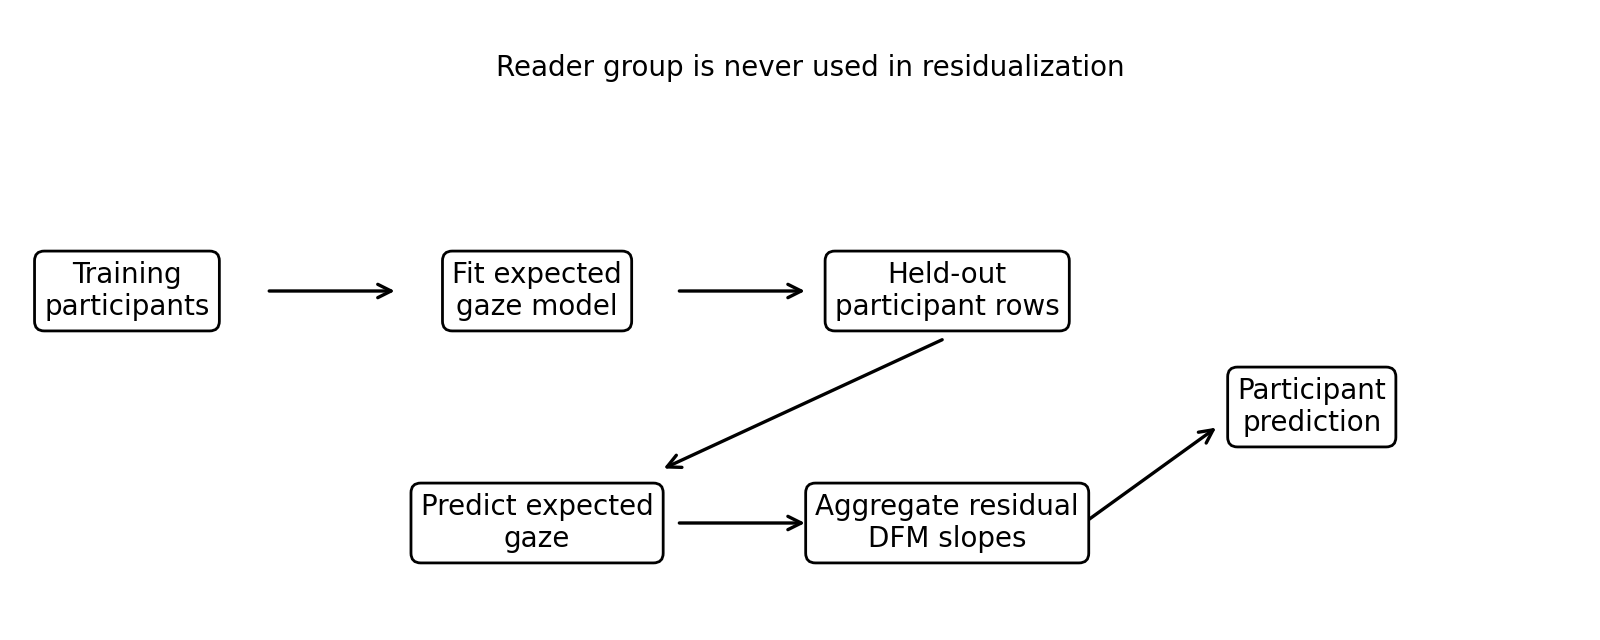
\includegraphics[width=0.92\linewidth]{figures/cross_fitted_residualization_schematic.png}
\caption{Cross-fitted residualization protects the held-out participant in each LOPO fold.}
\label{fig:crossfit-schematic}
\end{figure}
\begin{figure}[t]
\centering
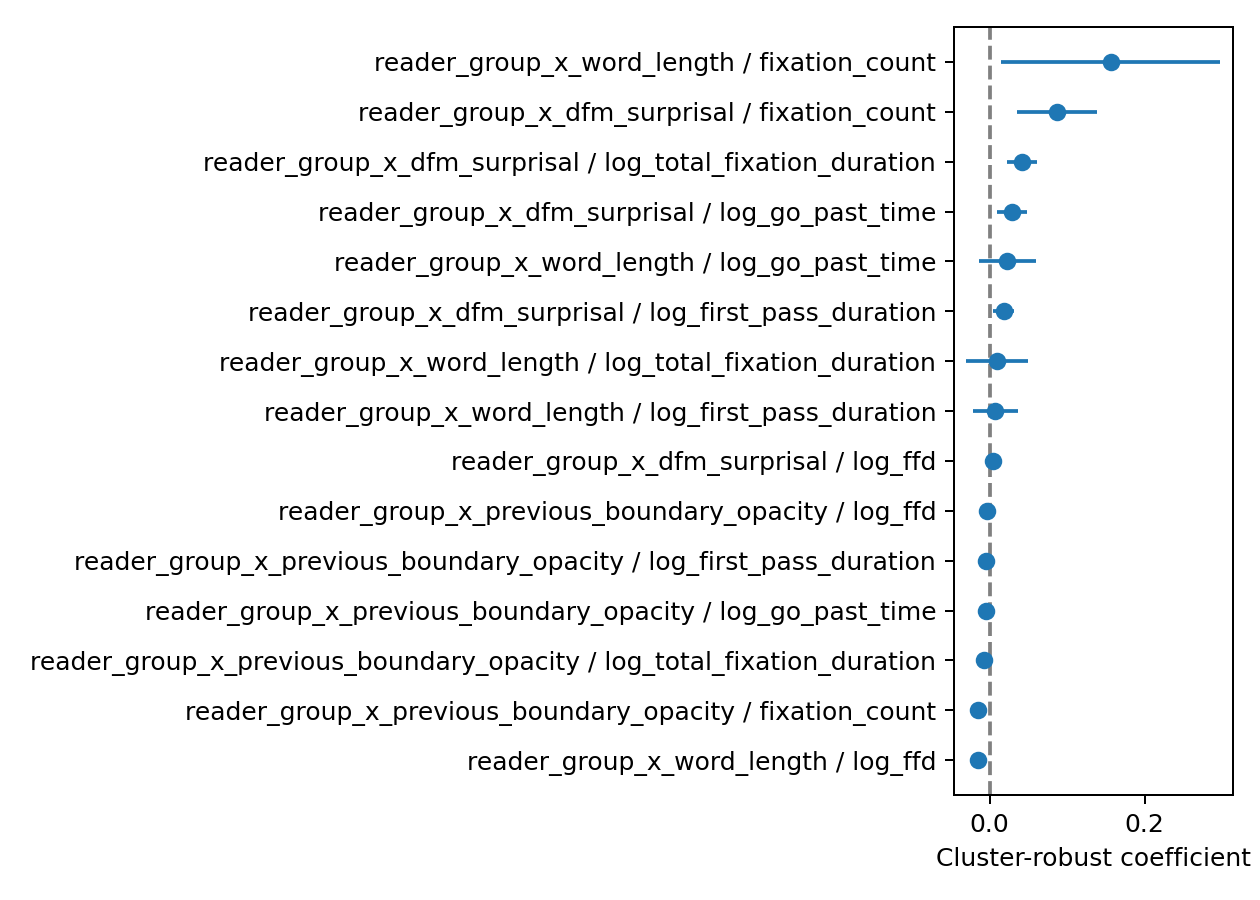
\includegraphics[width=0.92\linewidth]{figures/interaction_summary.png}
\caption{Focused reader-group interactions retained for interpretation, not model selection.}
\label{fig:interaction-summary}
\end{figure}
\begin{figure}[t]
\centering
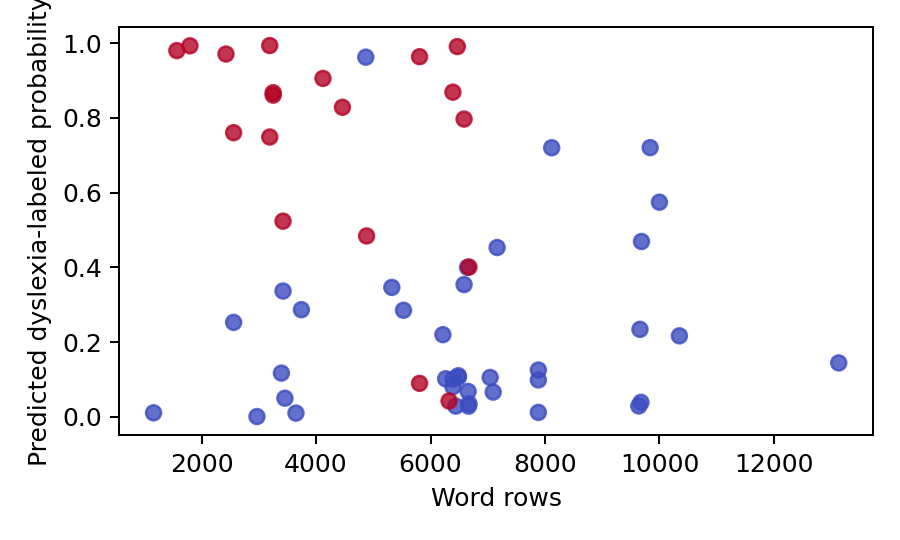
\includegraphics[width=0.92\linewidth]{figures/text_exposure_audit.png}
\caption{Text-exposure audit for prediction scores and participant-level errors.}
\label{fig:text-exposure-audit}
\end{figure}
